%!TEX root = main.tex
\section{Overview}

TODO GIVE AN EXAMPLE FOR 1 ROBUSTNESS AND 2 ROBUSTNESS IN THE P LANGUAGE (EXPLAIN A LITTLE BIT THE SYNTAX)

TALK ABOUT THE MOST USUAL WAY OF SEEING THEM

TAKE SOME EXECUTIONS AND SHOW HOW THEY CAN BE REORDERED AND EXECUTED ON A STRONGER SEMANTICS

EXPLAIN THE STRONGER SEMANTICS

SAY THAT FINDING VIOLATIONS MEANS DETECTING SOME PARTICULAR CLASS OF CYCLES

SAY WHAT ARE THE CONSEQUENCES: SAFETY, DEADLOCK

SAY THAT FINDING SUCH CYCLES CAN BE DONE ON THE STRONGER SEMANTICS - GIVE THE MAIN IDEAS

\begin{figure}
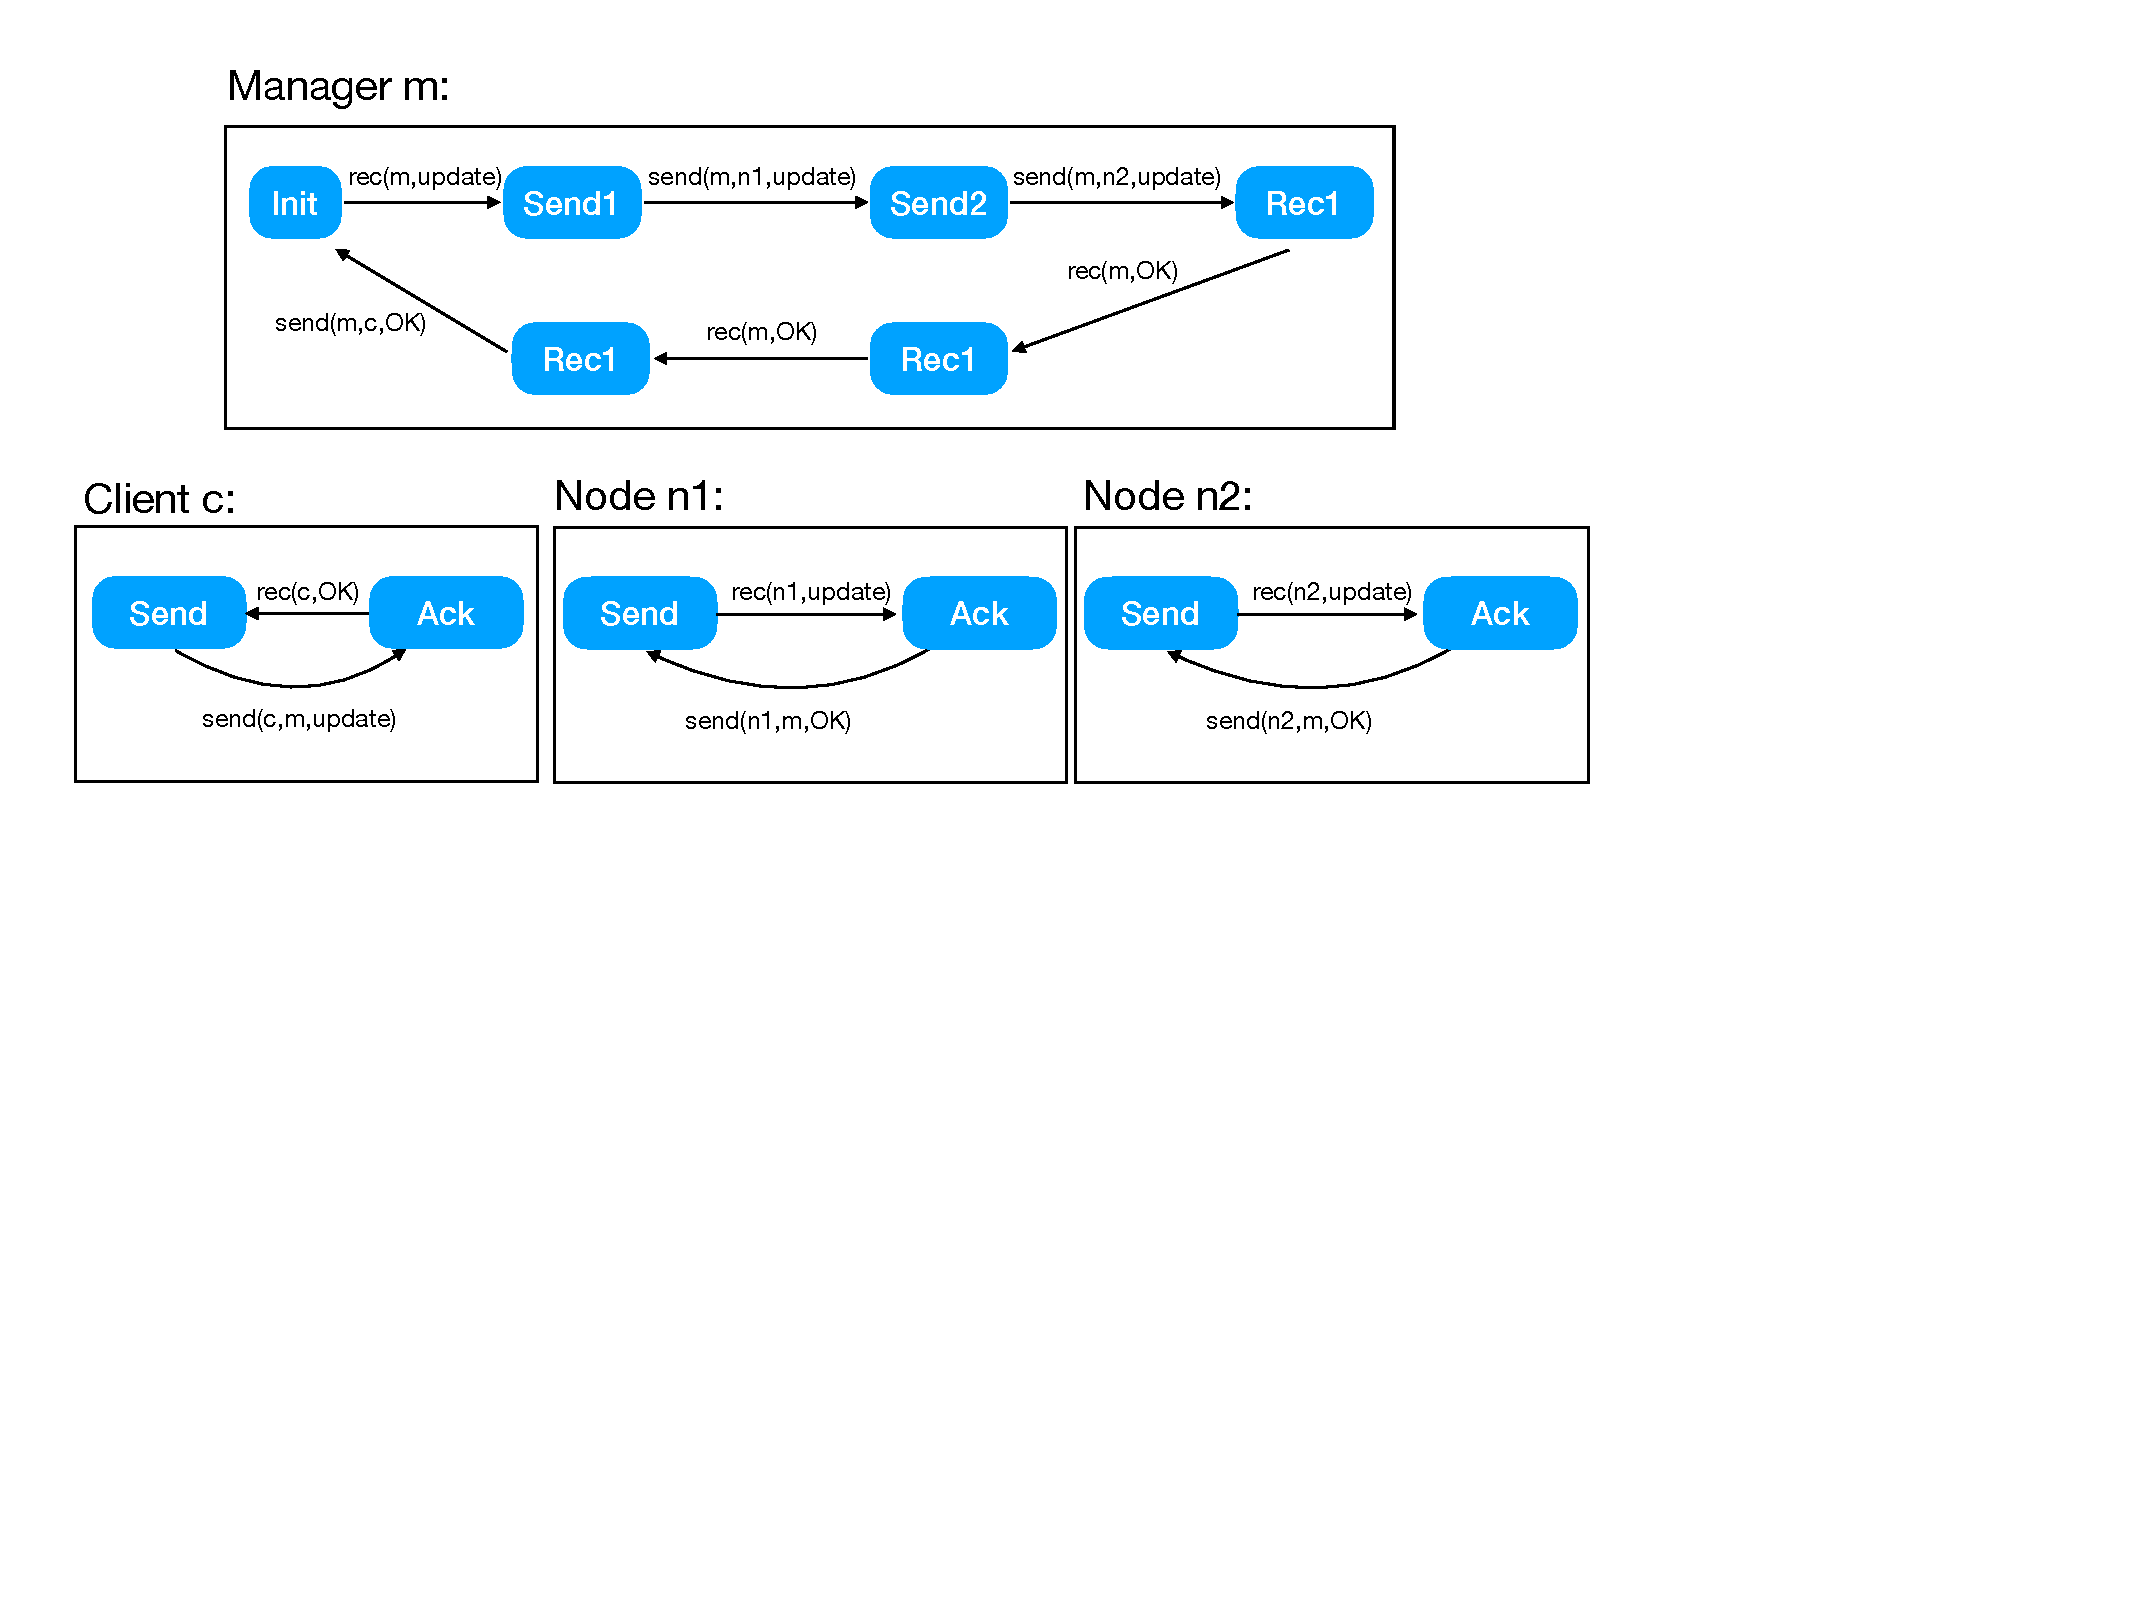
\includegraphics[width=10cm]{commit.pdf}
\caption{A distributed commit protocol.}
\label{fig:elevator}
\end{figure}

\begin{figure}
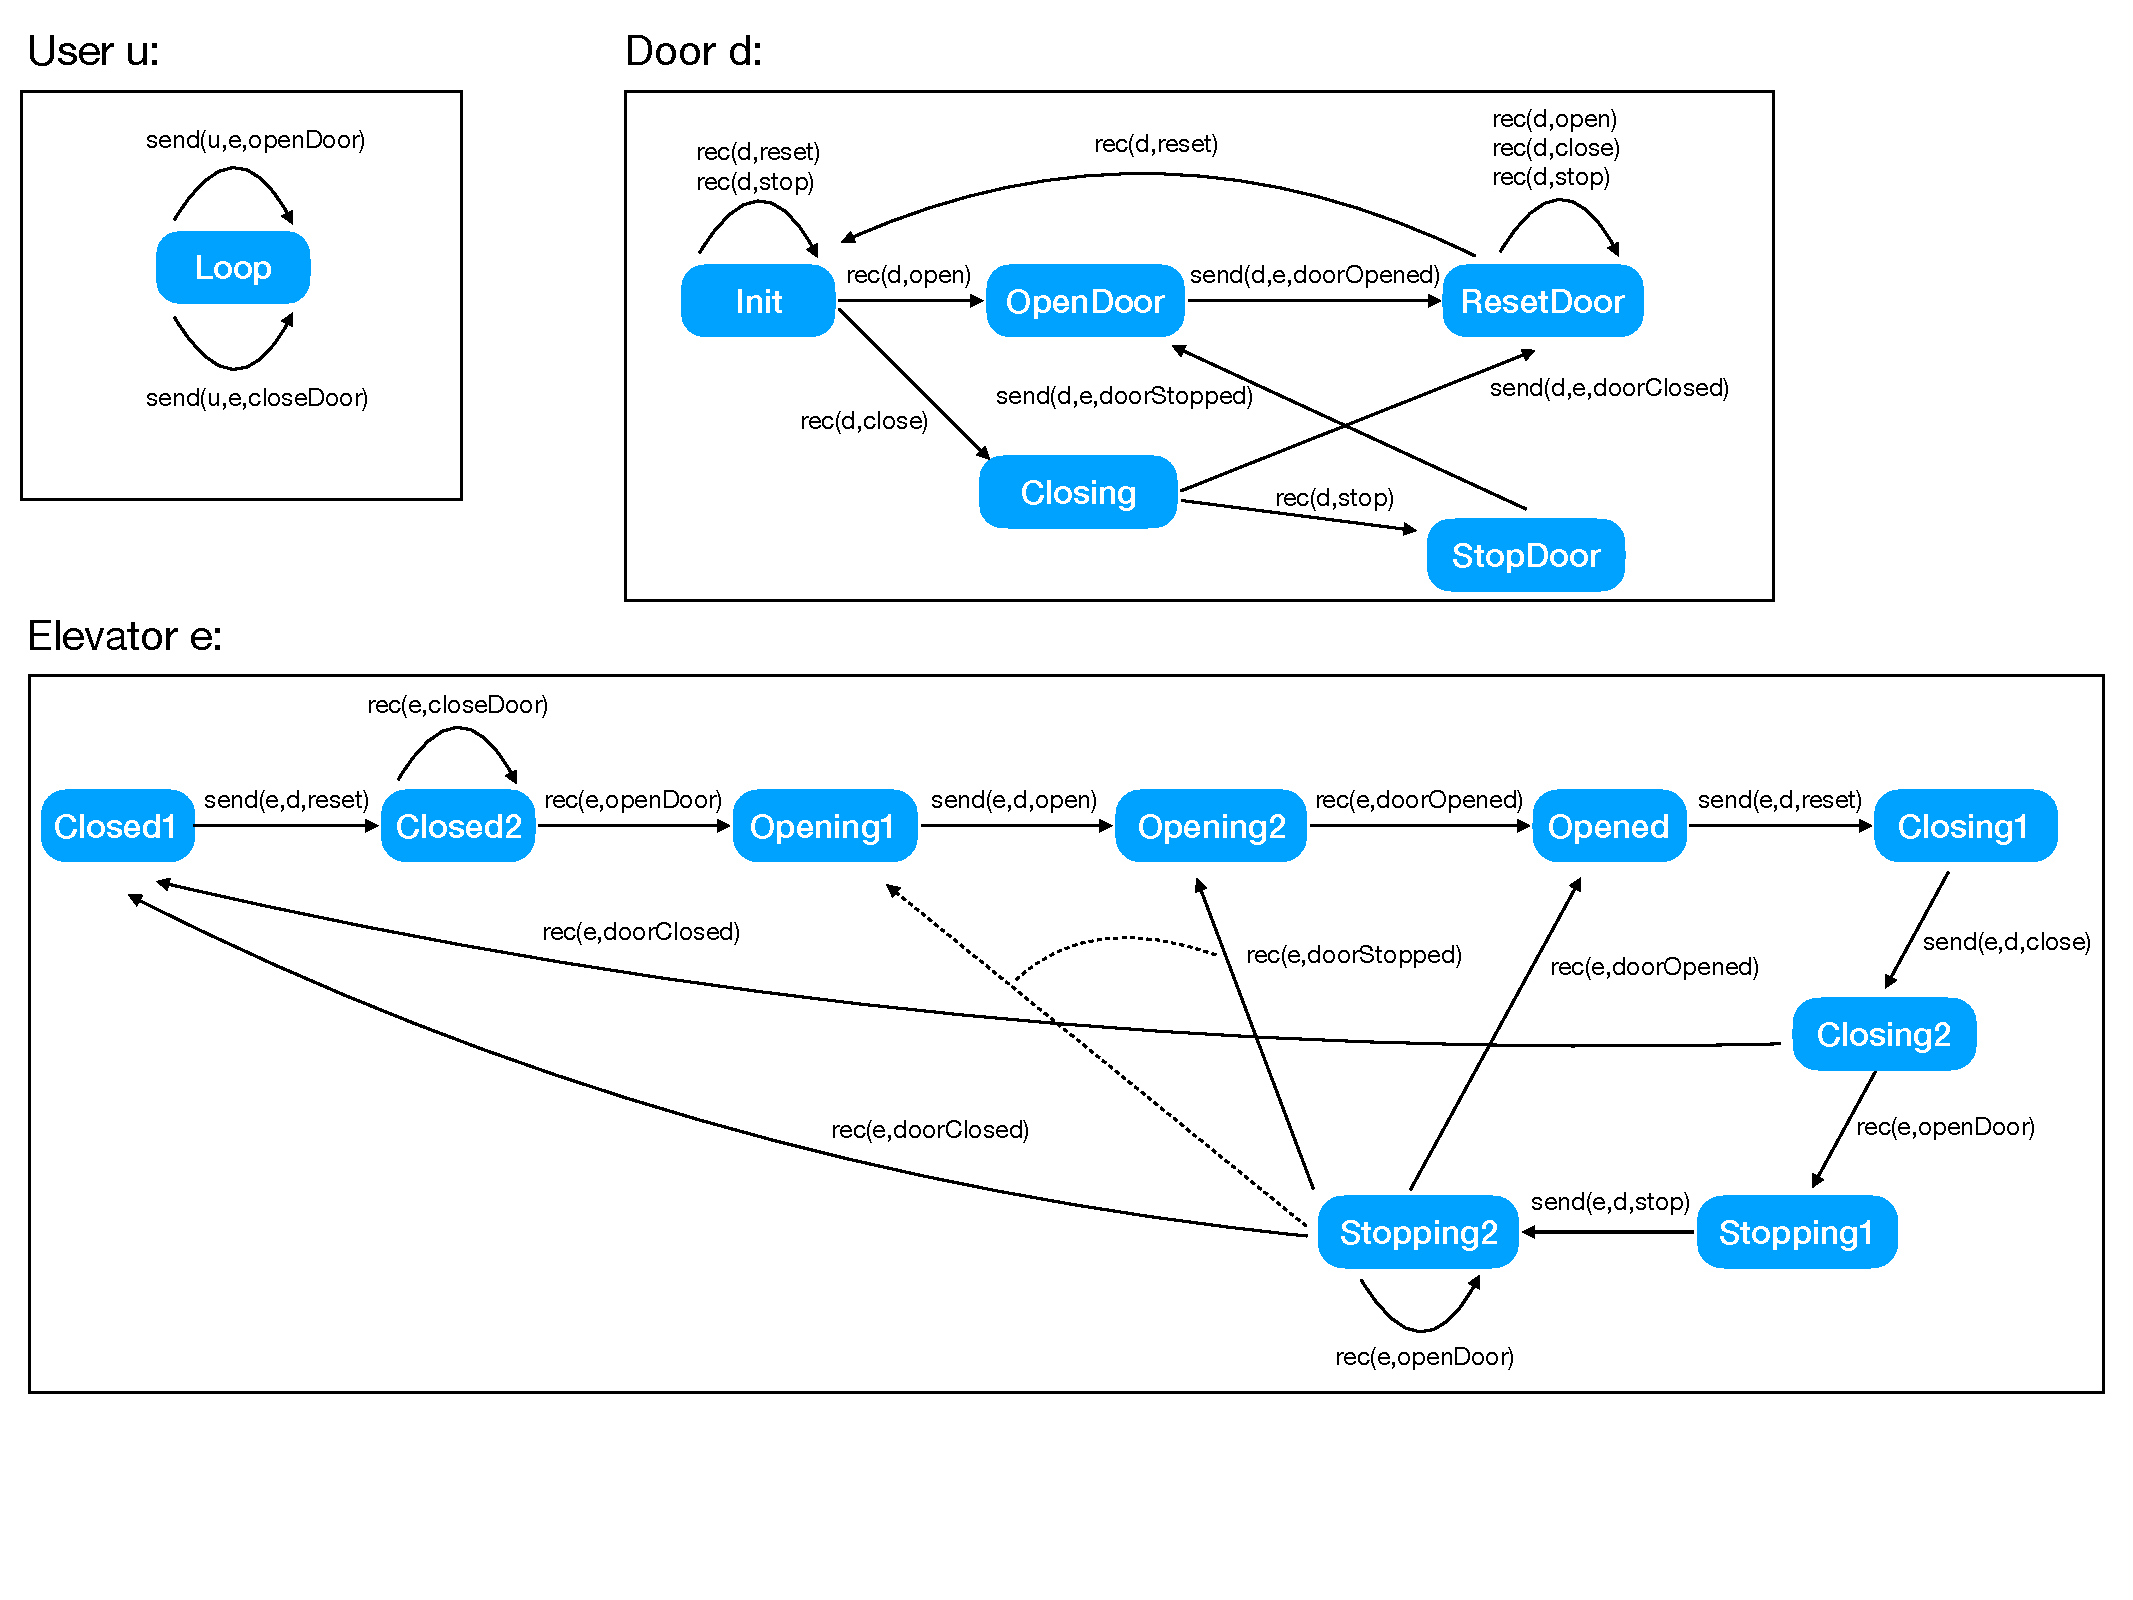
\includegraphics[width=13cm]{elevator.pdf}
\caption{The Elevator example}
\label{fig:elevator}
\end{figure}

\begin{figure}
\includegraphics[width=12cm]{german.pdf}
\caption{The German cache coherence protocol}
\label{fig:elevator}
\end{figure}

